\section{Performance}

\subsection{Module Testing}

\begin{figure}[hbt] 
\centering 
\includegraphics[width=1.0\columnwidth,keepaspectratio]{enc-chip.jpg}
\caption{Typical input noise on a single FSSR2 ASIC chip of an SVT module.}
\label{fig:enc-chip}
\end{figure} 

Detailed quality assurance procedures were developed for testing the modules during assembly at Fermilab,
reception tests at JLab, tracker integration, and commissioning. At each stage the results were compared with
previous measurements. The module performance was tested by the calibration procedures. No significant
correlated noise has been observed between the channels of the same chip, chips of the same module, or closely
placed modules. The measured average channel noise (see Fig.~\ref{fig:enc-chip}) is comparable with the
estimated contributions of different noise sources. The gain dispersion measured on the channels is within the
specifications of the readout chip (see Fig.~\ref{fig:gain-chip}). To verify operational stability and functionality
of the module at low temperature with active cooling, a performance and burn-in test was conducted at
-20$^\circ$C using a sealed container and a module in a carrier box, and the results were within the specifications.

\begin{figure}[hbt] 
\centering 
\includegraphics[width=1.0\columnwidth,keepaspectratio]{gain-chip.jpg}
\caption{Distribution of the gain for the channels of one representative FSSR2 ASIC.}
\label{fig:gain-chip}
\end{figure}

\begin{figure}[hbt] 
	\centering 
	\includegraphics[width=1.0\columnwidth,keepaspectratio]{encstriplength.png}
	\caption{Input noise vs. strip length of a typical FSSR2 ASIC. The results of a linear fit are shown.}
	\label{fig:encstriplength}
\end{figure}

Longer silicon strips have higher capacitance and thus a higher input noise (see Fig.~\ref{fig:encstriplength}).
Noise calibration accounts for the different strip lengths and pitch adapter layouts that affect the input
capacitance of the preamplifier. The mean noise values scale linearly with strip length, which confirms that the
noise is dominated by the strip capacitance and not by coherent noise pickup of the system. The channel noise has
a linear dependence on the strip length with an offset p$_0$ about 400 electrons (with shaper at 125~ns)
corresponding to the ENC for the shortest strips and a slope p$_1$ of 27 electrons, consistent with FSSR2 noise
measurements at comparable capacitive load taken on a single-chip test board with discrete capacitors (see
Fig.~\ref{fig:fssr2-enc-c}).

The equivalent noise charge of the SVT channels is shown in  Fig.~\ref{fig:enc}. The peak is $\sim$1600 electrons
(signal-to-noise ratio 15), the shoulder on the left side is related to the shorter strips. The channel noise allows
setting a 3$\sigma$ threshold at the 30~keV level. 

\begin{figure}[hbt] 
	\centering 
	\includegraphics[width=1.0\columnwidth,keepaspectratio]{enc.png}
	\caption{SVT ENC for all channels. The main peak corresponds to the full length strips (33~cm). The shoulder
          on the left side is related to the shorter strips.}
	\label{fig:enc}
\end{figure}

The detector response and full readout chain calibration was done with $\gamma$ and $\beta$ sources, cosmic
muons, an electron beam, and a proton beam. The output from the 3-bit ADC does not allow for a good resolution
of the pulse height. To increase the number of bins in the cluster charge distribution, a sliding window method was
used, combining the data taken for the same time window in several runs with discriminator thresholds set for the
required binning. When using signals from minimum-ionizing particles, like cosmic rays or a $^{90}$Sr $\beta$
source, the signal distribution is fit with a Landau-Gauss convolution. The detector response to a MIP was about
24000 electrons, which is what is expected for the 320-$\mu$m thick sensor. The results of absolute gain
calibration with a $\gamma$ source (Am$^{241}$) are shown in Fig.~\ref{fig:signal-gamma}. The signal peak is in
good agreement with the expected position (marked with an arrow). 

\begin{figure}[hbt] 
	\centering 
	\includegraphics[width=1.0\columnwidth,keepaspectratio]{signal-gamma.jpg}
	\caption{Signal from Am$^{241}$ $\gamma$ source. The results of a Gaussian fit are shown and the
          expected peak position is marked with an arrow.}
	\label{fig:signal-gamma}
\end{figure}

\subsection{Integration and System Checkout}

To verify the performance of the integrated detector, data acquisition chain, power services, and cooling system, as
well as the detector control and data acquisition software, the final detector system was installed in the clean room
and used at all stages of tracker integration and commissioning. The SVT was operated for several months under
environmental conditions close to those in Hall~B. Defects known before the integration of the system were
reestablished. 99.9\% of channels were operational after the detector integration. 
 
\begin{figure}[hbt] 
\centering 
\includegraphics[width=0.8\columnwidth,keepaspectratio]{occupancy-threshold.jpg}
\caption{Log occupancy vs. DAC hit/no-hit threshold (in DAC bins) squared . The results of a linear fit are shown.}
\label{fig:occupancy-threshold}
\end{figure}

The noise behavior was found to be within expectations and well understood. The dependence of the noise on the
environmental temperature and humidity is small and the noise performance in Hall~B was comparable with the
results taken in the clean room during integration. Several diagnostic tools were used to measure the
common-mode noise performance of the detector. The noise occupancy plot with no charge injection was used to find
the noise value. This plot probes the tail of the noise distribution, which can show effects that are masked by the
higher occupancy at low thresholds and provides a cross-check of the noise value obtained from the response curve
measurement. A Most Probable Value (MPV) of the signal peak from a MIP corresponds to the 100$^{th}$ DAC bin.
Figure~\ref{fig:occupancy-threshold} shows the log occupancy vs. threshold squared plot. Purely Gaussian noise
gives a straight line in the plot. Occupancy refers to the normalized total number of hits in all channels in a run.
The power of this plot is to show non-Gaussian noise contributions as deviations from this linear fall-off. The hit
map is plotted in the plane spanned by channel number and event number. It is an important diagnostic tool to test
for the presence of the correlated noise and to understand the data quality, such as dead/noisy channels, channel
occupancy, uniformity across the channels and events in a run, and coherent effects on the channels in individual
events.

\begin{figure}[hbt] 
\centering 
\includegraphics[width=1.0\columnwidth,keepaspectratio]{svt_gain.jpg}
\caption{Distribution of gain for the SVT channels. The results of a Gaussian fit are shown.}
\label{fig:svt_gain}
\end{figure}

No significant correlated noise has been observed between the channels of the same chip, between the chips of
the same module, or between the closely placed modules. The front-end electronics performed reliably, and no
chip failures were observed. The distribution of gain was uniform and stable for all channels (see
Fig.~\ref{fig:svt_gain}). 
 
\begin{figure}[hbt] 
\centering 
\includegraphics[width=1.0\columnwidth,keepaspectratio]{svt-hall.jpg}
\caption{SVT installed in Hall~B before being integrated with the CLAS12 detector. The cables are routed
  through the slots in the support flange. The cooling pipes, insulated with  foam, are attached to the bottom
  of the support tube.}
\label{fig:svt-hall}
\end{figure}

In the hall the SVT was dismounted from the integration cart, craned to the target level in the horizontal
position using the mounting brackets on the support tube and a counter-weight system to balance the weight of
the cables, which remained connected to the modules and coiled around the support tube during this operation.
The support tube was attached to the Central Vertex Tracker service cart with the alignment system for final
adjustment of the SVT along the beamline. The cart hosts the crates for the power supplies, back-end electronics,
slow controls, and the dry air distribution system. The service cart can be moved along the beamline on rails,
providing access to the detector during maintenance. The power, network, gas, and cooling lines are long enough
to allow the cart to be moved up to 5~m upstream of the nominal SVT installation position. Figure~\ref{fig:svt-hall}
shows the SVT detector after installation in Hall~B. The SVT Faraday cage, insulated with foam, can be seen on the
right side of the photograph. All modules were found to be fully functional after transportation from the assembly
site and installation on the beamline. 

\begin{figure}[hbt] 
\centering 
\includegraphics[width=1.0\columnwidth,keepaspectratio]{hybrid-temps.png}
\caption{Hybrid temperatures (left) and the difference in temperature between the two sides of the modules
  with the coolant at -26$^\circ$C (right).}
\label{fig:hybrid-temps}
\end{figure}

The SVT barrel has no direct silicon temperature measurements. The spatially closest information available is
from the temperature sensors on each side of the HFCB (between the FSSR2 chips) and from the ambient sensors
on the upstream ring in the outer regions (see Fig.~\ref{fig:ambient-sensors}). The temperature variation of the
SVT modules measured by sensors mounted on the hybrids with the coolant at -26$^\circ$C is shown in
Fig.~\ref{fig:hybrid-temps} (left). In these operating conditions the module temperatures were uniformly
distributed within the region, with lower temperatures close to the cooling lines. The Region~3 temperatures were
slightly higher than in the inner regions due to the design of the cold plate and longer lengths of the heat sinks
(double-peak structure of the distribution). The temperature difference between the two sides of a module is
within 1$^\circ$C as shown in Fig.~\ref{fig:hybrid-temps} (right). The leakage current is extremely sensitive to
temperature, doubling every $\sim$8$^\circ$C~\cite{SZE}. Sensor leakage currents remained at the same
low levels after installation (see Fig.~\ref{fig:currents}). The spread in the distribution of the leakage currents
is due to variations in sensor temperatures. Thermal cycling of the modules verified the robustness of the bond
wires.

\begin{figure}[hbt] 
\centering 
\includegraphics[width=1.0\columnwidth,keepaspectratio]{currents.jpg}
\caption{Sensor leakage currents after detector integration. The spread in the distribution of the leakage currents
  is due to variations in the sensor temperatures.}
\label{fig:currents}
\end{figure}

\subsection{Commissioning with Cosmic Rays}

Cosmic ray tests of the SVT have been used to check track reconstruction routines for the SVT, to qualify the
geometrical precision of the detector assembly by track-based alignment methods, to establish the correct
readout, to verify good noise performance, to study the full response for the entire detector, to measure the
inter-strip couplings, and to study the time evolution of the detector response. Once the reception tests of the
first assembled modules were complete, a cosmic test stand was assembled (see Fig.~\ref{fig:cosmic-stand}) to
verify the expected performance of the detector. Four SVT modules were stacked vertically between the two
trigger plastic scintillator counters. Each scintillator was equipped with a photomultiplier tube (PMT) on one side.
Evaluation of the signal-to-noise ratio and capacitive coupling confirmed the estimates and validated the full
readout chain calibration data.

\begin{figure}[hbt] 
\centering 
\includegraphics[width=1.0\columnwidth,keepaspectratio]{cosmic-stand.jpg}
\caption{The SVT cosmic test stand. Four SVT modules in their carrier boxes are mounted between the trigger
  paddles.}
\label{fig:cosmic-stand}
\end{figure}

Cosmic data during detector integration in the clean room were taken in a stand-alone mode using the
self-triggering feature of the FSSR2 readout chip in coincidence logic. VSCM boards reading the SVT modules
located at the top and bottom halves of the horizontally placed barrel provided the trigger signals via the signal
distribution of two VXS crates. The coincidence of  signals from the trigger interface boards of both crates was
taken as the cosmic trigger. With the logic described the trigger rate was $\sim$10~Hz. The response of the
channels was uniform, and the performance results obtained during tracker integration were confirmed. The
angular distribution of the cosmic muons reconstructed in the SVT is shown in Fig.~\ref{fig:track-phi-theta}, where
$\theta$ is the polar angle and $\phi$ is the azimuthal angle. The tracks are uniformly distributed within the
acceptance.

\begin{figure}[hbt] 
\centering 
\includegraphics[width=1.0\columnwidth,keepaspectratio]{track-phi-theta.jpg}
\caption{Angular distribution of the cosmic muons reconstructed in the SVT.}
\label{fig:track-phi-theta}
\end{figure}

After installation of the SVT in Hall~B and checkout of the detector services and readout system, a trigger
from the Central Time-of-Flight (CTOF) detector~\cite{ctof-nim} (located radially outward of the SVT) was
used to collect cosmic data for the CLAS12 Central Detector. A cosmic muon reconstructed in the Central
Detector is shown in Fig.~\ref{fig:cd-cosmic-event}. The SVT is the inner detector, surrounded by the Barrel
Micromegas Tracker (BMT)~\cite{mm-nim}, the CTOF, and the Central Neutron Detector (CND)~\cite{cnd-nim}.
The yellow circles represent crosses (matched hits on both sides of a module) in the SVT and the green circles
correspond to the clusters in the BMT. Both tracking detectors have the same number of layers. The SVT has
small angle stereo strips on the two sides of each module, and the BMT has interleaving layers of strips along
the beam axis and arcs at fixed radii. Between the physics data taking runs more cosmic trigger data were
collected for alignment, calibration, and performance studies.  A hit map for the SVT channels during the cosmic
run is shown in Fig.~\ref{fig:cosmic-hitmap-svt}. Several sensors were under-depleted, visible on the plot as
channels with higher occupancy. The lower hit occupancy on the right side of the map is due to the shorter strips. 

\begin{figure}[hbt] 
\centering 
\includegraphics[width=0.6\columnwidth,keepaspectratio]{cd-cosmic-event.png}
\caption{Cosmic muon reconstructed in the CLAS12 Central Detector as seen in the CLAS12 Event Display
  ({\it ced}). The track is matched to the signal registered in the CTOF and the CND.}
\label{fig:cd-cosmic-event}
\end{figure}

\begin{figure}[hbt] 
\centering 
\includegraphics[width=1.0\columnwidth,keepaspectratio]{cosmic-hitmap-svt.png}
\caption{Monitoring SVT hit map during a cosmic run showing sensor module vs. strip number (channel). The strips
  on the right side have shorter length.}
\label{fig:cosmic-hitmap-svt}
\end{figure}

The cluster size is affected by electronics cross-talk independent of the position where the charge was generated,
and charge sharing among neighboring strips depending on the position where the charge was deposited. The
charge sharing among two adjacent strips was studied using the $\eta$-function (also referred to as the response
function), defined for the 2-strip clusters as the ratio of the pulse height of the left strip to the pulse height of
the cluster, independently of which strip has the higher charge (seed strip). Figure~\ref{fig:eta-function} shows
the  $\eta$-function obtained from the measurement of on-track clusters from cosmic muons. The distribution
was obtained without applying cuts on the selected tracks. The granularity of the pulse height after the digitization
is coarse due to the 3-bit ADC of the readout chip. The area where charge sharing occurs is large. There is a
pronounced peak in the center between the two readout strips where all of the charge is collected by the
intermediate strip. Because of capacitive coupling, signals on these intermediate strips are partially transferred to
the readout strips.

\begin{figure}[hbt] 
\centering 
\includegraphics[width=1.0\columnwidth,keepaspectratio]{eta-function.png}
\caption{Charge sharing in the SVT sensor: $\eta$-function for the two-strip clusters (see text for details).}
\label{fig:eta-function}
\end{figure}

The cluster size has been studied as a function of the local track angle. For normally incident tracks, the charge
is shared at most between the two adjacent strips, although due to diffusion a small amount of charge may be
collected by neighboring strips. The strip multiplicity of the clusters (cluster size) in a cosmic run is shown in
Fig.~\ref{fig:cluster-size}. The size of the clusters is lowest in the innermost region and increases with radius
due to a larger local track angle (the tracks, triggered by the CTOF, crossing the barrel far from the beamline).
The few very wide clusters observed are attributed to muons with high energy, generating a shower in the
detector. The results are in agreement with simulations and the data on the charge sharing among adjacent
readout strips obtained during laser studies.

\begin{figure}[hbt] 
\centering 
\includegraphics[width=0.8\columnwidth,keepaspectratio]{cluster-size.png}
\caption{Strip multiplicity of the clusters in a cosmic run. The mean cluster size is in agreement with the simulated
  data.}
\label{fig:cluster-size}
\end{figure}

Cosmic muons are an important source for calibration and alignment. Their trajectories are sensitive to
misalignments of the different tracker parts. The cosmic muons significantly improve the alignment precision. A
preliminary alignment of the SVT was done using a sample of several million cosmic muon tracks taken without
solenoid magnetic field. With exception of the modules located at shallow angles to the vertical axis, the acquired
sample provided adequate statistics for the tracks to extract the misalignment data. The tracks crossing the
sensors at large inclination angles and low-energy tracks subject to multiple scattering were rejected. An additional
requirement on the $\chi^2$ per degree of freedom of the track fit was applied to reject tracks affected by
outlier hits. The spatial residuals before (blue) and after (red) the alignment procedure (see
Fig.~\ref{fig:alignment}) are shown. Only the shifts in the sensor plane were taken into account in the alignment
procedure for this plot. Validation of the alignment procedures was performed on Monte Carlo simulation and cosmic
data.

\begin{figure}[hbt] 
\centering 
\includegraphics[width=0.9\columnwidth,keepaspectratio]{alignment.jpg}
\caption{Validation of alignment procedures on cosmic data. Residuals for one of the SVT sensors before (left
  peak) and after (right peak) alignment.}
\label{fig:alignment}
\end{figure}

\subsection{Commissioning with Beam}

The performance of an SVT module was studied at Fermilab in a beam test with 120~GeV protons. The SVT module
in the plastic carrier box was mounted vertically behind the CMS pixel beam telescope (8 planes,
$\approx$6~$\mu$m track position uncertainty, 2~cm $\times$ 2~cm active area), which was used as the trigger
and the tracker. The beam test setup is shown in Fig.~\ref{fig:beam-test}. The production SVT DAQ was exercised
at different event rates. The event block mode was tested up to 100k protons per 4~s spill with no busy time. The
signal-to-noise ratio was in agreement with the results with radioactive sources and cosmic muons. Several millions
triggers were taken at different discriminator thresholds. The measured cluster charge distribution is shown in
Fig.~\ref{fig:cluster-charge-protons}.  The expected position resolution of the silicon sensors was confirmed. 

\begin{figure}[hbt] 
\centering 
\includegraphics[width=0.8\columnwidth,keepaspectratio]{beam-test.png}
\caption{Beam test setup at Fermilab. The SVT module in the plastic carrier box is mounted vertically downstream
  from the beam telescope. The hybrid side in on the top and the copper insert is attached to a water-cooled heatsink.}
\label{fig:beam-test}
\end{figure}

\begin{figure}[h] 
\centering 
\includegraphics[width=1.0\columnwidth,keepaspectratio]{cluster-charge-protons.png}
\caption{Cluster charge distribution from 120~GeV protons. The expected MPV of the peak for a MIP is indicated
  by the arrow.}
\label{fig:cluster-charge-protons}
\end{figure}

The front-end electronics performance and noise occupancy of the detector were studied during physics data
taking. No interference with other CLAS12 subsystems was found. The data quality and detector operational
stability  were verified with both online and offline monitoring packages. There were occasional FSSR2 chip
latch-ups observed after the start of a new run. These latch-ups were traced to improper configuration settings
of the chips and were fixed by adding additional resets to the run start sequence.

\begin{figure}[h] 
\centering 
\includegraphics[width=0.6\columnwidth,keepaspectratio]{cd-tracks.jpg}
\caption{Multi-track event reconstructed in the CLAS12 Central Detector during a beam run as seen in the CLAS12
  Event Display ({\it ced}).}
\label{fig:cd-tracks}
\end{figure}

Tracks reconstructed in the CLAS12 Central Detector during a physics run are shown in Fig.~\ref{fig:cd-tracks}.
The level-1 trigger latency is finely tuned to match the CLAS12 trigger delays. Single Event Monitor (SEM) error
checking implemented in the VSCM firmware allows real-time monitoring of the readout errors induced by the
radiation. Relatively minor single event upsets were recorded in the SVT readout electronics with no latch-ups or
single event burn-outs observed. The SEM recorded events are correlated with beam conditions in Hall~B during
the run. The SVT readout and power supply crates did not require rebooting. No readout or data corruption issues
were observed~\cite{SEENOTE}. 

\begin{figure}[htb] 
\centering 
\includegraphics[width=1.0\columnwidth,keepaspectratio]{svt-hit-timing.jpg}
\caption{SVT hit timing in ns referenced to the CTOF hit time in a physics run with the liquid-hydrogen target.}
\label{fig:svt-hit-timing}
\end{figure}

The FSSR2 readout chip does not provide the timing information from the hit. Reading the time stamp associated
with a hit was implemented in the VSCM board. The time stamp is synchronized with the "Got Hit" pulse from the
chip when the pulse height reaches the threshold set for the first discriminator of the ADC. Timing of the SVT
hits referenced to the CTOF timing are shown in Fig.~\ref{fig:svt-hit-timing}. The data correspond to the time
difference between the SVT and the CTOF time stamps for the SVT hits that were associated with a track.
Applying a cut on this time difference can be  used to remove background and noise hits in the track-seeding
algorithm.

Radiation-induced energy levels in the middle of the band gap cause an increase in the number of thermally
generated electron-hole pairs. Consequently the bulk sensor leakage current increases with the absorbed flux
according to the empirical parameterization depending on the fluence, annealing time $t$, temperature during
annealing $T_A$, and reference temperature $T_{ref}$ as:

\begin{equation} \Delta I_R = \alpha(t, T_{ref}, T_A)\Phi{V} \label{eq:leakage-fluence},
\end{equation}
where $\Phi$ is the particle fluence, $V$ is the volume of the sensor, and
$\alpha \approx$ 4$\cdot$10$^{-17}$~A/cm after 80~min annealing at 60$^\circ$C~\cite{DIERLAMMTHESIS}.
The raised leakage current increases the noise and heats up the sensor, which, in turn, will further increase the
leakage current. When the temperature increases beyond a critical temperature where the cooling cannot maintain
a stable temperature, this will result in thermal runaway. A feedback self-heating loop has to be counteracted with
sufficient cooling. Figure~\ref{fig:thermal-runaway} shows thermal runaway in the two innermost layers of the SVT
that received the highest radiation dose after beam operation. The leakage currents in other layers were stable.
The monitoring data were taken after a physics run with a liquid-hydrogen target, when there was no beam in the
hall for extended time. The leakage currents became stable when the coolant temperature was decreased.

\begin{figure}[hbt] 
\centering 
\includegraphics[width=1.0\columnwidth,keepaspectratio]{thermal-runaway.jpg}
\caption{Thermal runaway in the SVT inner layers (L1 and L2). The data shown correspond to the period right after
  the physics run, when the beam was turned off.}
\label{fig:thermal-runaway}
\end{figure}

Figure~\ref{fig:leakage-layers-deuterium} shows monitoring plots for the average sensor leakage currents in the
SVT layers during data-taking with a liquid-deuterium target. For the first few hours in the time period shown there
was no beam in the hall and the currents were stable. Currents in all layers increase with time when beam is present.
The jumps in the leakage current of a layer between two values are related to beam trips. The largest difference
between the beam-on and beam-off levels and the rate of current increase is in the inner layers. The distribution of
leakage currents is in agreement with the accumulated dose, with higher currents in the sensors closest to the
target. The sensors in the outermost layer have higher temperatures, affecting the currents. The data were taken at
a 50~nA election beam current. For the unirradiated sensors, the lowest leakage currents were in Region~1, where
heatsinks have the shortest length.

\begin{figure}[hbt] 
\centering 
\includegraphics[width=1.0\columnwidth,keepaspectratio]{leakage-layers-deuterium.png}
\caption{Monitoring plots of the sensor leakage currents in the SVT layers during a run with a liquid-deuterium
  target.}
\label{fig:leakage-layers-deuterium}
\end{figure}

Comparison of the rates of leakage current increase with different targets is shown in
Fig.~\ref{fig:leakage-hydrogen-deuterium}. The rate of current increase with a liquid-deuterium target was about
1~nA per hour. The rate for a liquid-hydrogen target was 0.06 nA per hour. The difference in rates can be
attributed to the higher neutron flux in the CLAS12 Central Detector for the liquid-deuterium target. The increase
of leakage current when beam is delivered to the target is also larger for the liquid-deuterium target. The data were
taken at 50~nA beam current corresponding to the instantaneous luminosity of
0.7~$\times$10$^{35}$~cm$^{-2}$s$^{-1}$ per nucleon. The leakage current for the run with a liquid-hydrogen target
is higher because it was taken after the run with a liquid-deuterium target.

\begin{figure}[hbt] 
\centering 
\includegraphics[width=1.0\columnwidth,keepaspectratio]{leakage-hydrogen-deuterium.png}
\caption{Average sensor leakage currents in the SVT layer~1 during runs with liquid-hydrogen and liquid-deuterium
  targets. There was no beam for the first few hours for the liquid-deuterium target.}
\label{fig:leakage-hydrogen-deuterium}
\end{figure}

\begin{figure}[hbt] 
\centering 
\includegraphics[width=1.0\columnwidth,keepaspectratio]{hit-map-rga.png}
\caption{SVT hit map during a physics run with the liquid-hydrogen target.}
\label{fig:hit-map-rga}
\end{figure}

The surface of the silicon sensors suffers from damage due to ionizing radiation. The damage affects the insulating
properties of the SiO$_2$ layer between the strips and the aluminum electrodes that collect the charge generated
by the photons and the charged particles. The trapped positive charge causes an accumulation of electrons in the
Si/SiO$_2$ interface between the strips, thus decreasing the resistance between the strips and increasing the
interstrip capacitance, which affects noise performance and degrades the spatial resolution. After a year of running,
several sensors developed pinholes (strips with DC current through the damaged dielectric between aluminum strip
and implant, resulting in a high current flowing into a channel) observed as groups of adjacent hot channels. The
performance of the charge amplifying chip is deteriorated by the high current flowing into a channel. The bias
voltage on these sensors (high occupancy regions on the map) has been lowered to reduce the noise and the
abnormally high strip leakage currents. High current going through the bias resistor could cause unsafe voltage on
the input of the preamplifier if the coupling capacitor is damaged. The increased leakage current was reduced by
decreasing the detector temperature. The sensors are kept below -10$^\circ$C to freeze the reverse annealing,
interleaved with short periods at room temperature for the beneficial annealing. A hit map of the SVT from a beam
run is shown in Fig.~\ref{fig:hit-map-rga}. Sensors with pinholes are seen on the map as darker horizontal lines due
to reduced efficiency (under-depleted sensors) with strips of masked hot channels with no hits. In the absence of
physics background the same sensors in Fig.~\ref{fig:cosmic-hitmap-svt} showed higher occupancy because the
average hit multiplicity in the cosmic event is low. 

\begin{figure}[hbt] 
\centering 
\includegraphics[width=1.0\columnwidth,keepaspectratio]{mean-hit-occupancy.png}
\caption{Average number of hits for the sectors of the innermost SVT layer with a 5-cm long liquid-hydrogen
  target at 50~nA beam current.}
\label{fig:mean-hit-occupancy}
\end{figure}

Figure~\ref{fig:mean-hit-occupancy} shows the average hit occupancy (number of hits) per event in the innermost
SVT layer for the data taken with a liquid-hydrogen target at a beam current of 50~nA. The hits are uniformly
distributed among the sectors with occupancies close to 1\% (each sensor has 256 strips).

\begin{figure}[hbt] 
\centering 
\includegraphics[width=1.0\columnwidth,keepaspectratio]{hit-occupancy-shielding.jpg}
\caption{Hit occupancies with and without the 51~$\mu$m-thick tungsten shield installed outside of the target
  scattering chamber.}
\label{fig:hit-occupancy-shielding}
\end{figure}

The impact of the tungsten shield on the SVT occupancy (see Section~\ref{sec:simdetails}) is shown in
Fig.~\ref{fig:hit-occupancy-shielding}. The occupancies in all SVT layers are substantially lower, which results in
better tracking performance due to reduced combinatorics. The effect of the shield on momentum resolution is
negligible~\cite{SHIELDNOTE}. For the liquid-hydrogen target the occupancy in the innermost layer of the SVT
is approximately 1\%, decreasing to 0.5\% in the outermost layer. There is no hit efficiency loss due to the dead
time of the readout system at such occupancies.

\begin{figure}[hbt] 
\centering 
\includegraphics[width=1.0\columnwidth,keepaspectratio]{beam-no-beam-occupancy.png}
\caption{SVT hit multiplicity during a liquid-hydrogen run at 50~nA beam current. The narrow peak on the left
  side represents the SVT occupancy with no beam.}
\label{fig:beam-no-beam-occupancy}
\end{figure}

The noise performance of the SVT during physics data taking is demonstrated in
Fig.~\ref{fig:beam-no-beam-occupancy}, showing the SVT hit multiplicity during a liquid-hydrogen run at a 50~nA
beam current. The main peak is at about 130 hits per event, which corresponds to 0.6\% detector occupancy.
The peak on the left side represents the SVT occupancy when there was no beam in the hall obtained with a
random trigger. The plot confirms a good signal-to-noise ratio of the detector. 

\begin{figure}[hbt] 
\centering 
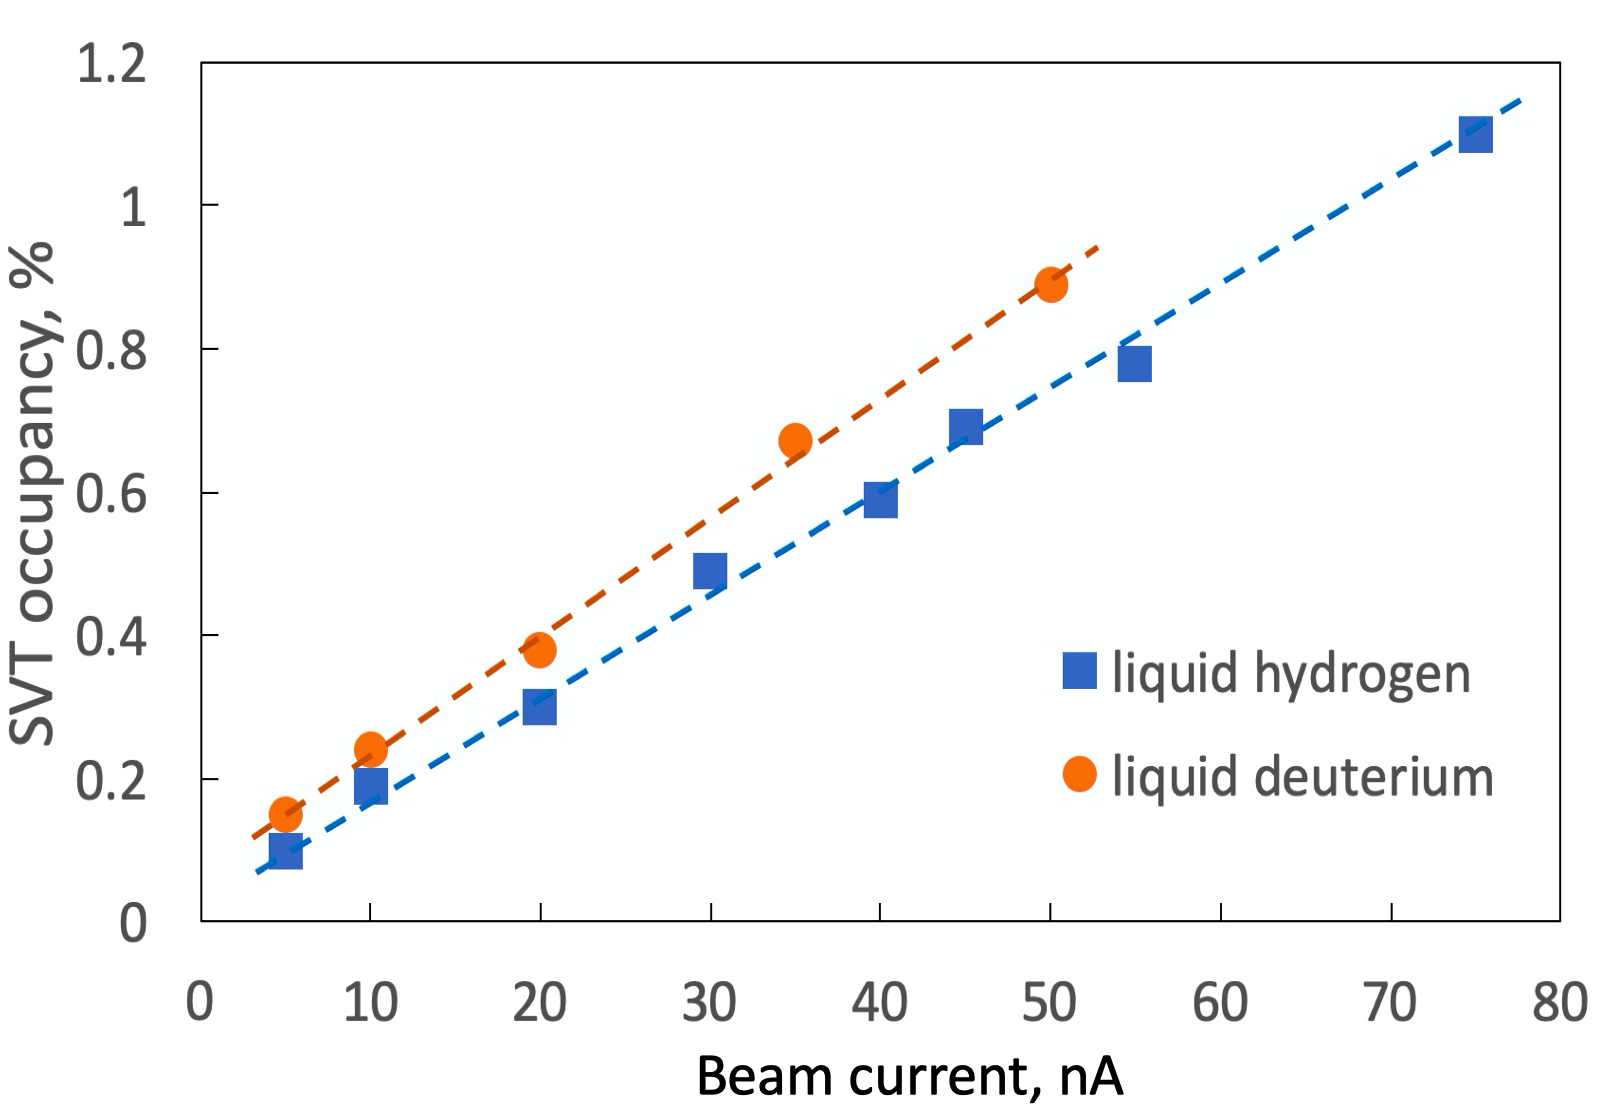
\includegraphics[width=1.0\columnwidth,keepaspectratio]{occupancy-beam-current.png}
\caption{SVT occupancy vs. beam current for the liquid-hydrogen and deuterium targets.}
\label{fig:occupancy-beam-current}
\end{figure}

Figure~\ref{fig:occupancy-beam-current} shows the SVT occupancy vs. beam current for the liquid-hydrogen and
deuterium targets. The production data were taken at 50~nA. The SVT occupancy increases linearly with luminosity
and remains at low levels not causing a substantial drop in the track finding efficiency.

\begin{figure}[hbt] 
\centering 
\includegraphics[width=1.0\columnwidth,keepaspectratio]{residual.jpg}
\caption{Centroid residual for one of the SVT sensors after preliminary tracker alignment. The results of a
  Gaussian fit are shown.}
\label{fig:residual}
\end{figure}

A series of dedicated Central Vertex Tracker alignment runs was done at low beam current without solenoid
magnetic field. New alignment data are collected whenever the position of the Central Detector subsystems or
the target has changed. The dependence of the residuals on the track parameters is explicitly taken into account.
The alignment code uses the partial derivatives of the Distance Of Closest Approach (DOCA) taken with respect
to the track parameters and the SVT geometry. This approach accounts for the correlated shifts among the
geometry parameters. In addition to the track-based alignment, the data from the mechanical survey of the
fiducials are also recorded whenever the detectors are moved. The centroid residual for one of the SVT sensors
after preliminary tracker alignment is shown in Fig.~\ref{fig:residual}. The sensor spatial resolution is within the
specifications. Further improvements are expected from the ongoing development of the alignment algorithm and
the track reconstruction code (like energy loss and Lorentz angle corrections that have strong impact on alignment).
See Ref.~\cite{recon-nim} for more information.

\begin{figure}[hbt] 
\centering 
\includegraphics[width=1.0\columnwidth,keepaspectratio]{lorentz-angle.jpg}
\caption{Cluster size vs. local track azimuthal angle. The insert shows the dependence of the cluster size on the
  track angle. The smallest cluster size corresponds to the Lorentz angle.}
\label{fig:lorentz-angle}
\end{figure}

In a strong magnetic field, charge in the silicon detector drifts at the Lorentz angle (the angle between the drift
direction and the electric field), which must be taken into account when reconstructing the cluster position.
Figure~\ref{fig:lorentz-angle} shows the average cluster size at different local azimuthal angles of the track. The
zero angle is related to normally incident tracks. The data were taken at negative polarity of the solenoid field. The
Lorentz angle $\theta_{LA}$ is independent of the track local angle and contributes to the charge spread among
the strips. There is no compensation for the Lorentz angle in the orientation of the SVT sensors to minimize the
cluster size for the tracks originating from the primary vertex. The Lorentz angle can be calculated as the track
incidence angle corresponding to the minimum of the average cluster size when the track local angle is equal to the
Lorentz angle.

\begin{figure}[hbt] 
\centering 
\includegraphics[width=0.8\columnwidth,keepaspectratio]{matched-hits.jpg}
\caption{Number of the SVT hits per track. For most tracks all 6 SVT layers have been matched.}
\label{fig:matched-hits}
\end{figure}

The number of matched SVT hits per reconstructed track in the physics run with the liquid-hydrogen target is
shown in Fig.~\ref{fig:matched-hits}. For most tracks all 6 SVT layers have been matched to a track. Tracks
with a low number of matched hits passed through the gaps between the modules.


\begin{figure}[hbt] 
\centering 
\includegraphics[width=1.0\columnwidth,keepaspectratio]{layer-efficiency.jpg}
\caption{Efficiency of hit matching in the SVT layers. The hit is matched if it is associated with a track and there
  are on-track hits in two adjacent layers.}
\label{fig:layer-efficiency}
\end{figure}

Figure~\ref{fig:layer-efficiency} shows the efficiency of matching the hits to the tracks in each SVT layer. For
each layer the efficiency is the ratio of the number of tracks with hits in the layer associated with a track to the
number of tracks with on-track hits in two adjacent layers. The lower efficiency in the outer SVT layer is due to
the tracks that are not within its acceptance. The data were taken at 5 nA beam current with a 5-cm-long
liquid-hydrogen target. The efficiencies are expected to improve with further development of the tracking and
alignment algorithms. 
